\documentclass{article}

%% Created with wxMaxima 16.04.0

\setlength{\parskip}{\medskipamount}
\setlength{\parindent}{0pt}
\usepackage[utf8]{inputenc}
\DeclareUnicodeCharacter{00B5}{\ensuremath{\mu}}
\usepackage{graphicx}
\usepackage{color}
\usepackage{amsmath}
\usepackage{ifthen}
\newsavebox{\picturebox}
\newlength{\pictureboxwidth}
\newlength{\pictureboxheight}
\newcommand{\includeimage}[1]{
    \savebox{\picturebox}{\includegraphics{#1}}
    \settoheight{\pictureboxheight}{\usebox{\picturebox}}
    \settowidth{\pictureboxwidth}{\usebox{\picturebox}}
    \ifthenelse{\lengthtest{\pictureboxwidth > .95\linewidth}}
    {
        \includegraphics[width=.95\linewidth,height=.80\textheight,keepaspectratio]{#1}
    }
    {
        \ifthenelse{\lengthtest{\pictureboxheight>.80\textheight}}
        {
            \includegraphics[width=.95\linewidth,height=.80\textheight,keepaspectratio]{#1}
            
        }
        {
            \includegraphics{#1}
        }
    }
}
\newlength{\thislabelwidth}
\DeclareMathOperator{\abs}{abs}
\usepackage{animate} % This package is required because the wxMaxima configuration option
                      % "Export animations to TeX" was enabled when this file was generated.

\definecolor{labelcolor}{RGB}{100,0,0}

\begin{document}
Show that it is possible to generate pythagorean type triples \$(x,y,z)\$ such that \$x\^{}2 + 2 y\^{}2 = z\^{}2\$.  Proceed by looking at the intersection of lines through \$(1,1)\$ and the ellipse \$x\^{}2 + 2 y\^{}2 = 3\$. The point \$(1,1)\$ is on the ellipse. The second intersection is at \$(u,v)\$ which depends on \$m\$ (the gradient of the line).  Writing \$m = a/b\$ gives expressions for \$x\$, \$y\$ and \$z\$ 


\noindent
%%%%%%%%%%%%%%%
%%% INPUT:
\begin{minipage}[t]{8ex}\color{red}\bf
(\%{}i16) 
\end{minipage}
\begin{minipage}[t]{\textwidth}\color{blue}
ya : 1 + m*(x-1);
\end{minipage}
%%% OUTPUT:
\[\displaystyle
\tag{ya}\label{ya}
m\,\left( x-1\right) +1\mbox{}
\]
%%%%%%%%%%%%%%%



\noindent
%%%%%%%%%%%%%%%
%%% INPUT:
\begin{minipage}[t]{8ex}\color{red}\bf
(\%{}i25) 
\end{minipage}
\begin{minipage}[t]{\textwidth}\color{blue}
crossings: solve([2*ya\^{}2 + x\^{}2 = 3], [x]);
\end{minipage}
%%% OUTPUT:
\[\displaystyle
\tag{crossings}\label{crossings}
[x=\frac{2{{m}^{2}}-4m-1}{2{{m}^{2}}+1},x=1]\mbox{}
\]
%%%%%%%%%%%%%%%


\noindent
%%%%%%%%%%%%%%%
%%% INPUT:
\begin{minipage}[t]{8ex}\color{red}\bf
(\%{}i26) 
\end{minipage}
\begin{minipage}[t]{\textwidth}\color{blue}
u: crossings[1];
\end{minipage}
%%% OUTPUT:
\[\displaystyle
\tag{u}\label{u}
x=\frac{2{{m}^{2}}-4m-1}{2{{m}^{2}}+1}\mbox{}
\]
%%%%%%%%%%%%%%%


\noindent
%%%%%%%%%%%%%%%
%%% INPUT:
\begin{minipage}[t]{8ex}\color{red}\bf
(\%{}i28) 
\end{minipage}
\begin{minipage}[t]{\textwidth}\color{blue}
v: ratsimp(m*(u-1) + 1);
\end{minipage}
%%% OUTPUT:
\[\displaystyle
\tag{v}\label{v}
mx-m+1=-\frac{2{{m}^{2}}+2m-1}{2{{m}^{2}}+1}\mbox{}
\]
%%%%%%%%%%%%%%%


\noindent
%%%%%%%%%%%%%%%
%%% INPUT:
\begin{minipage}[t]{8ex}\color{red}\bf
(\%{}i29) 
\end{minipage}
\begin{minipage}[t]{\textwidth}\color{blue}
ratsimp(u\^{}2);
\end{minipage}
%%% OUTPUT:
\[\displaystyle
\tag{\%{}o29}\label{o29} 
{{x}^{2}}=\frac{4{{m}^{4}}-16{{m}^{3}}+12{{m}^{2}}+8m+1}{4{{m}^{4}}+4{{m}^{2}}+1}\mbox{}
\]
%%%%%%%%%%%%%%%


\noindent
%%%%%%%%%%%%%%%
%%% INPUT:
\begin{minipage}[t]{8ex}\color{red}\bf
(\%{}i30) 
\end{minipage}
\begin{minipage}[t]{\textwidth}\color{blue}
ratsimp(v\^{}2);
\end{minipage}
%%% OUTPUT:
\[\displaystyle
\tag{\%{}o30}\label{o30} 
{{m}^{2}}\,{{x}^{2}}+\left( 2m-2{{m}^{2}}\right) x+{{m}^{2}}-2m+1=\frac{4{{m}^{4}}+8{{m}^{3}}-4m+1}{4{{m}^{4}}+4{{m}^{2}}+1}\mbox{}
\]
%%%%%%%%%%%%%%%


\noindent
%%%%%%%%%%%%%%%
%%% INPUT:
\begin{minipage}[t]{8ex}\color{red}\bf
(\%{}i44) 
\end{minipage}
\begin{minipage}[t]{\textwidth}\color{blue}
ratsimp(u\^{}2 + 2*v\^{}2);
\end{minipage}
%%% OUTPUT:
\[\displaystyle
\tag{\%{}o44}\label{o44} 
\left( 2{{m}^{2}}+1\right) \,{{x}^{2}}+\left( 4m-4{{m}^{2}}\right) x+2{{m}^{2}}-4m+2=3\mbox{}
\]
%%%%%%%%%%%%%%%


\noindent
%%%%%%%%%%%%%%%
%%% INPUT:
\begin{minipage}[t]{8ex}\color{red}\bf
(\%{}i32) 
\end{minipage}
\begin{minipage}[t]{\textwidth}\color{blue}
ratsimp(subst(m = a/b, u));
\end{minipage}
%%% OUTPUT:
\[\displaystyle
\tag{\%{}o32}\label{o32} 
x=-\frac{{{b}^{2}}+4ab-2{{a}^{2}}}{{{b}^{2}}+2{{a}^{2}}}\mbox{}
\]
%%%%%%%%%%%%%%%


\noindent
%%%%%%%%%%%%%%%
%%% INPUT:
\begin{minipage}[t]{8ex}\color{red}\bf
(\%{}i33) 
\end{minipage}
\begin{minipage}[t]{\textwidth}\color{blue}
ratsimp(subst(m = a/b, v));
\end{minipage}
%%% OUTPUT:
\[\displaystyle
\tag{\%{}o33}\label{o33} 
\frac{ax+b-a}{b}=\frac{{{b}^{2}}-2ab-2{{a}^{2}}}{{{b}^{2}}+2{{a}^{2}}}\mbox{}
\]
%%%%%%%%%%%%%%%


\noindent
%%%%%%%%%%%%%%%
%%% INPUT:
\begin{minipage}[t]{8ex}\color{red}\bf
(\%{}i45) 
\end{minipage}
\begin{minipage}[t]{\textwidth}\color{blue}
X: 2*a\^{}2 - 4*a*b - b\^{}2;
\end{minipage}
%%% OUTPUT:
\[\displaystyle
\tag{X}\label{X}
-{{b}^{2}}-4ab+2{{a}^{2}}\mbox{}
\]
%%%%%%%%%%%%%%%


\noindent
%%%%%%%%%%%%%%%
%%% INPUT:
\begin{minipage}[t]{8ex}\color{red}\bf
(\%{}i46) 
\end{minipage}
\begin{minipage}[t]{\textwidth}\color{blue}
Y: b\^{}2-2*a*b-2*a\^{}2;
\end{minipage}
%%% OUTPUT:
\[\displaystyle
\tag{Y}\label{Y}
{{b}^{2}}-2ab-2{{a}^{2}}\mbox{}
\]
%%%%%%%%%%%%%%%


\noindent
%%%%%%%%%%%%%%%
%%% INPUT:
\begin{minipage}[t]{8ex}\color{red}\bf
(\%{}i47) 
\end{minipage}
\begin{minipage}[t]{\textwidth}\color{blue}
Z: b\^{}2+2*a\^{}2;
\end{minipage}
%%% OUTPUT:
\[\displaystyle
\tag{Z}\label{Z}
{{b}^{2}}+2{{a}^{2}}\mbox{}
\]
%%%%%%%%%%%%%%%


\noindent
%%%%%%%%%%%%%%%
%%% INPUT:
\begin{minipage}[t]{8ex}\color{red}\bf
(\%{}i48) 
\end{minipage}
\begin{minipage}[t]{\textwidth}\color{blue}
ratsimp(X\^{}2 + 2*Y\^{}2);
\end{minipage}
%%% OUTPUT:
\[\displaystyle
\tag{\%{}o48}\label{o48} 
3{{b}^{4}}+12{{a}^{2}}\,{{b}^{2}}+12{{a}^{4}}\mbox{}
\]
%%%%%%%%%%%%%%%


\noindent
%%%%%%%%%%%%%%%
%%% INPUT:
\begin{minipage}[t]{8ex}\color{red}\bf
(\%{}i50) 
\end{minipage}
\begin{minipage}[t]{\textwidth}\color{blue}
ratsimp(3*Z\^{}2);
\end{minipage}
%%% OUTPUT:
\[\displaystyle
\tag{\%{}o50}\label{o50} 
3{{b}^{4}}+12{{a}^{2}}\,{{b}^{2}}+12{{a}^{4}}\mbox{}
\]
%%%%%%%%%%%%%%%


\noindent
%%%%%%%%%%%%%%%
%%% INPUT:
\begin{minipage}[t]{8ex}\color{red}\bf
(\%{}i23) 
\end{minipage}
\begin{minipage}[t]{\textwidth}\color{blue}
wxplot2d([sqrt((3 - x\^{}2)/2), -sqrt((3 - x\^{}2)/2)], [x,-3,3],
 [gnuplot\_postamble, "set zeroaxis;"])\$
\end{minipage}
%%% OUTPUT:
\[\displaystyle
\mbox{}\\\mbox{plot2d: expression evaluates to non-numeric value somewhere in plotting range.}\mbox{}\\\mbox{plot2d: expression evaluates to non-numeric value somewhere in plotting range.}\mbox{}\]
\[\displaystyle
\]
\[\tag{\%{}t23}\label{t23} 
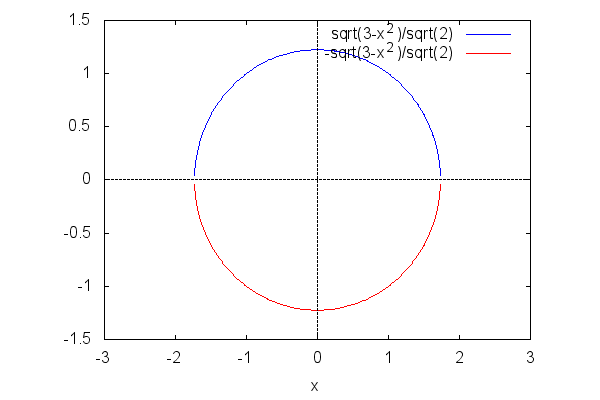
\includegraphics[width=.95\linewidth,height=.80\textheight,keepaspectratio]{weissman_2_img/weissman_2_1}\mbox{}
\]
%%%%%%%%%%%%%%%
\end{document}
